% Options for packages loaded elsewhere
\PassOptionsToPackage{unicode}{hyperref}
\PassOptionsToPackage{hyphens}{url}
\PassOptionsToPackage{dvipsnames,svgnames,x11names}{xcolor}
%
\documentclass[
  12,
  letterpaper,
  DIV=11,
  numbers=noendperiod]{scrartcl}

\usepackage{amsmath,amssymb}
\usepackage{iftex}
\ifPDFTeX
  \usepackage[T1]{fontenc}
  \usepackage[utf8]{inputenc}
  \usepackage{textcomp} % provide euro and other symbols
\else % if luatex or xetex
  \usepackage{unicode-math}
  \defaultfontfeatures{Scale=MatchLowercase}
  \defaultfontfeatures[\rmfamily]{Ligatures=TeX,Scale=1}
\fi
\usepackage{lmodern}
\ifPDFTeX\else  
    % xetex/luatex font selection
  \setmainfont[]{Times New Roman}
\fi
% Use upquote if available, for straight quotes in verbatim environments
\IfFileExists{upquote.sty}{\usepackage{upquote}}{}
\IfFileExists{microtype.sty}{% use microtype if available
  \usepackage[]{microtype}
  \UseMicrotypeSet[protrusion]{basicmath} % disable protrusion for tt fonts
}{}
\usepackage{xcolor}
\setlength{\emergencystretch}{3em} % prevent overfull lines
\setcounter{secnumdepth}{-\maxdimen} % remove section numbering
% Make \paragraph and \subparagraph free-standing
\ifx\paragraph\undefined\else
  \let\oldparagraph\paragraph
  \renewcommand{\paragraph}[1]{\oldparagraph{#1}\mbox{}}
\fi
\ifx\subparagraph\undefined\else
  \let\oldsubparagraph\subparagraph
  \renewcommand{\subparagraph}[1]{\oldsubparagraph{#1}\mbox{}}
\fi

\usepackage{color}
\usepackage{fancyvrb}
\newcommand{\VerbBar}{|}
\newcommand{\VERB}{\Verb[commandchars=\\\{\}]}
\DefineVerbatimEnvironment{Highlighting}{Verbatim}{commandchars=\\\{\}}
% Add ',fontsize=\small' for more characters per line
\usepackage{framed}
\definecolor{shadecolor}{RGB}{241,243,245}
\newenvironment{Shaded}{\begin{snugshade}}{\end{snugshade}}
\newcommand{\AlertTok}[1]{\textcolor[rgb]{0.68,0.00,0.00}{#1}}
\newcommand{\AnnotationTok}[1]{\textcolor[rgb]{0.37,0.37,0.37}{#1}}
\newcommand{\AttributeTok}[1]{\textcolor[rgb]{0.40,0.45,0.13}{#1}}
\newcommand{\BaseNTok}[1]{\textcolor[rgb]{0.68,0.00,0.00}{#1}}
\newcommand{\BuiltInTok}[1]{\textcolor[rgb]{0.00,0.23,0.31}{#1}}
\newcommand{\CharTok}[1]{\textcolor[rgb]{0.13,0.47,0.30}{#1}}
\newcommand{\CommentTok}[1]{\textcolor[rgb]{0.37,0.37,0.37}{#1}}
\newcommand{\CommentVarTok}[1]{\textcolor[rgb]{0.37,0.37,0.37}{\textit{#1}}}
\newcommand{\ConstantTok}[1]{\textcolor[rgb]{0.56,0.35,0.01}{#1}}
\newcommand{\ControlFlowTok}[1]{\textcolor[rgb]{0.00,0.23,0.31}{#1}}
\newcommand{\DataTypeTok}[1]{\textcolor[rgb]{0.68,0.00,0.00}{#1}}
\newcommand{\DecValTok}[1]{\textcolor[rgb]{0.68,0.00,0.00}{#1}}
\newcommand{\DocumentationTok}[1]{\textcolor[rgb]{0.37,0.37,0.37}{\textit{#1}}}
\newcommand{\ErrorTok}[1]{\textcolor[rgb]{0.68,0.00,0.00}{#1}}
\newcommand{\ExtensionTok}[1]{\textcolor[rgb]{0.00,0.23,0.31}{#1}}
\newcommand{\FloatTok}[1]{\textcolor[rgb]{0.68,0.00,0.00}{#1}}
\newcommand{\FunctionTok}[1]{\textcolor[rgb]{0.28,0.35,0.67}{#1}}
\newcommand{\ImportTok}[1]{\textcolor[rgb]{0.00,0.46,0.62}{#1}}
\newcommand{\InformationTok}[1]{\textcolor[rgb]{0.37,0.37,0.37}{#1}}
\newcommand{\KeywordTok}[1]{\textcolor[rgb]{0.00,0.23,0.31}{#1}}
\newcommand{\NormalTok}[1]{\textcolor[rgb]{0.00,0.23,0.31}{#1}}
\newcommand{\OperatorTok}[1]{\textcolor[rgb]{0.37,0.37,0.37}{#1}}
\newcommand{\OtherTok}[1]{\textcolor[rgb]{0.00,0.23,0.31}{#1}}
\newcommand{\PreprocessorTok}[1]{\textcolor[rgb]{0.68,0.00,0.00}{#1}}
\newcommand{\RegionMarkerTok}[1]{\textcolor[rgb]{0.00,0.23,0.31}{#1}}
\newcommand{\SpecialCharTok}[1]{\textcolor[rgb]{0.37,0.37,0.37}{#1}}
\newcommand{\SpecialStringTok}[1]{\textcolor[rgb]{0.13,0.47,0.30}{#1}}
\newcommand{\StringTok}[1]{\textcolor[rgb]{0.13,0.47,0.30}{#1}}
\newcommand{\VariableTok}[1]{\textcolor[rgb]{0.07,0.07,0.07}{#1}}
\newcommand{\VerbatimStringTok}[1]{\textcolor[rgb]{0.13,0.47,0.30}{#1}}
\newcommand{\WarningTok}[1]{\textcolor[rgb]{0.37,0.37,0.37}{\textit{#1}}}

\providecommand{\tightlist}{%
  \setlength{\itemsep}{0pt}\setlength{\parskip}{0pt}}\usepackage{longtable,booktabs,array}
\usepackage{calc} % for calculating minipage widths
% Correct order of tables after \paragraph or \subparagraph
\usepackage{etoolbox}
\makeatletter
\patchcmd\longtable{\par}{\if@noskipsec\mbox{}\fi\par}{}{}
\makeatother
% Allow footnotes in longtable head/foot
\IfFileExists{footnotehyper.sty}{\usepackage{footnotehyper}}{\usepackage{footnote}}
\makesavenoteenv{longtable}
\usepackage{graphicx}
\makeatletter
\def\maxwidth{\ifdim\Gin@nat@width>\linewidth\linewidth\else\Gin@nat@width\fi}
\def\maxheight{\ifdim\Gin@nat@height>\textheight\textheight\else\Gin@nat@height\fi}
\makeatother
% Scale images if necessary, so that they will not overflow the page
% margins by default, and it is still possible to overwrite the defaults
% using explicit options in \includegraphics[width, height, ...]{}
\setkeys{Gin}{width=\maxwidth,height=\maxheight,keepaspectratio}
% Set default figure placement to htbp
\makeatletter
\def\fps@figure{htbp}
\makeatother

\usepackage{booktabs}
\usepackage{longtable}
\usepackage{array}
\usepackage{multirow}
\usepackage{wrapfig}
\usepackage{float}
\usepackage{colortbl}
\usepackage{pdflscape}
\usepackage{tabu}
\usepackage{threeparttable}
\usepackage{threeparttablex}
\usepackage[normalem]{ulem}
\usepackage{makecell}
\usepackage{xcolor}
\KOMAoption{captions}{tableheading}
\makeatletter
\makeatother
\makeatletter
\makeatother
\makeatletter
\@ifpackageloaded{caption}{}{\usepackage{caption}}
\AtBeginDocument{%
\ifdefined\contentsname
  \renewcommand*\contentsname{Table of contents}
\else
  \newcommand\contentsname{Table of contents}
\fi
\ifdefined\listfigurename
  \renewcommand*\listfigurename{List of Figures}
\else
  \newcommand\listfigurename{List of Figures}
\fi
\ifdefined\listtablename
  \renewcommand*\listtablename{List of Tables}
\else
  \newcommand\listtablename{List of Tables}
\fi
\ifdefined\figurename
  \renewcommand*\figurename{Figure}
\else
  \newcommand\figurename{Figure}
\fi
\ifdefined\tablename
  \renewcommand*\tablename{Table}
\else
  \newcommand\tablename{Table}
\fi
}
\@ifpackageloaded{float}{}{\usepackage{float}}
\floatstyle{ruled}
\@ifundefined{c@chapter}{\newfloat{codelisting}{h}{lop}}{\newfloat{codelisting}{h}{lop}[chapter]}
\floatname{codelisting}{Listing}
\newcommand*\listoflistings{\listof{codelisting}{List of Listings}}
\makeatother
\makeatletter
\@ifpackageloaded{caption}{}{\usepackage{caption}}
\@ifpackageloaded{subcaption}{}{\usepackage{subcaption}}
\makeatother
\makeatletter
\@ifpackageloaded{tcolorbox}{}{\usepackage[skins,breakable]{tcolorbox}}
\makeatother
\makeatletter
\@ifundefined{shadecolor}{\definecolor{shadecolor}{rgb}{.97, .97, .97}}
\makeatother
\makeatletter
\makeatother
\makeatletter
\makeatother
\ifLuaTeX
  \usepackage{selnolig}  % disable illegal ligatures
\fi
\IfFileExists{bookmark.sty}{\usepackage{bookmark}}{\usepackage{hyperref}}
\IfFileExists{xurl.sty}{\usepackage{xurl}}{} % add URL line breaks if available
\urlstyle{same} % disable monospaced font for URLs
\hypersetup{
  pdftitle={Beer Preferences for Thursday Night Football: A Blanced Incomplete Block Design Experiment},
  pdfauthor={Matthew Murnane; Ethan Newcomb},
  colorlinks=true,
  linkcolor={blue},
  filecolor={Maroon},
  citecolor={Blue},
  urlcolor={Blue},
  pdfcreator={LaTeX via pandoc}}

\title{Beer Preferences for Thursday Night Football: A Blanced
Incomplete Block Design Experiment}
\author{Matthew Murnane \and Ethan Newcomb}
\date{}

\begin{document}
\maketitle
\ifdefined\Shaded\renewenvironment{Shaded}{\begin{tcolorbox}[interior hidden, frame hidden, borderline west={3pt}{0pt}{shadecolor}, breakable, enhanced, sharp corners, boxrule=0pt]}{\end{tcolorbox}}\fi

\newpage

\begin{center}
\textbf{\Large Abstract}
\end{center}

\newpage

\begin{center}
\textbf{\Large Introduction}
\end{center}

\newpage

\begin{center}
\textbf{\Large Methods}
\end{center}

\newpage

\begin{center}
\textbf{\Large Results}
\end{center}

\begin{longtable}[]{@{}cccccc@{}}
\caption{Beer Ratings by Participant}\tabularnewline
\toprule\noalign{}
Beers & Nolan & Jon & Beni & Zach & Row Means \\
\midrule\noalign{}
\endfirsthead
\toprule\noalign{}
Beers & Nolan & Jon & Beni & Zach & Row Means \\
\midrule\noalign{}
\endhead
\bottomrule\noalign{}
\endlastfoot
Sierra(Pale\_ale) & NA & 5.5 & 7 & 2.5 & 5.00 \\
Coors(Generic) & 6 & 6 & NA & 6.5 & 6.17 \\
Guinness(Dark) & 5.5 & 3.5 & 4 & NA & 4.33 \\
Pliny(IPA) & 3 & NA & 8.5 & 2 & 4.50 \\
Column Means & 4.83 & 5 & 6.5 & 3.67 & NA \\
\end{longtable}

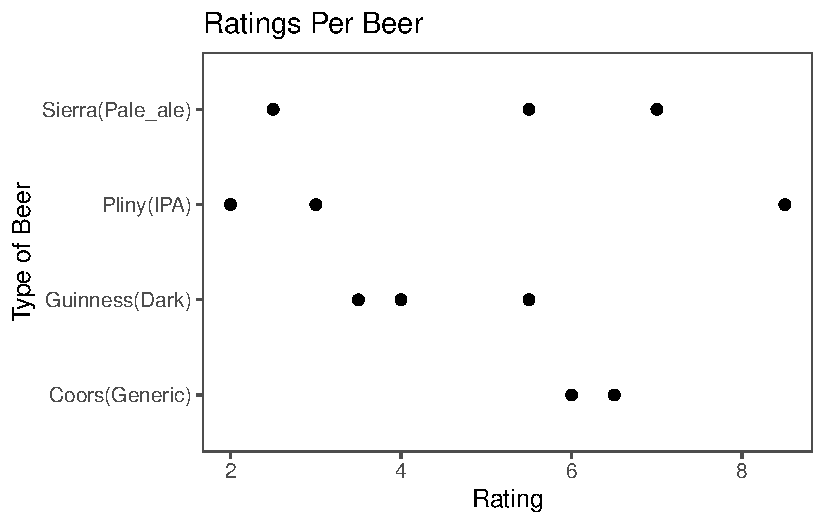
\includegraphics{BIBD_beer_preferences_files/figure-pdf/unnamed-chunk-3-1.pdf}

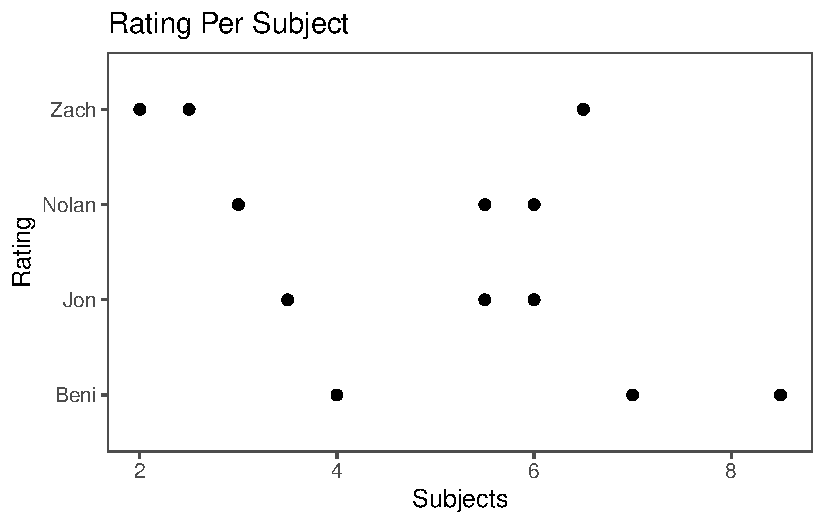
\includegraphics{BIBD_beer_preferences_files/figure-pdf/unnamed-chunk-4-1.pdf}

\begin{longtable}[]{@{}lrrrrr@{}}
\caption{ANOVA Table for Linear Model}\tabularnewline
\toprule\noalign{}
& Df & Sum Sq & Mean Sq & F value & Pr(\textgreater F) \\
\midrule\noalign{}
\endfirsthead
\toprule\noalign{}
& Df & Sum Sq & Mean Sq & F value & Pr(\textgreater F) \\
\midrule\noalign{}
\endhead
\bottomrule\noalign{}
\endlastfoot
names & 3 & 12.16667 & 4.055556 & 1.197212 & 0.4001761 \\
beers & 3 & 14.39583 & 4.798611 & 1.416564 & 0.3414684 \\
Residuals & 5 & 16.93750 & 3.387500 & NA & NA \\
\end{longtable}

\newpage

\begin{center}
\textbf{\Large Conclusion}
\end{center}

\newpage

\begin{center}
\textbf{\Large Appendix}
\end{center}

\hypertarget{code-used}{%
\section{Code Used}\label{code-used}}

\hypertarget{libraries-used}{%
\subsubsection{Libraries Used}\label{libraries-used}}

\begin{Shaded}
\begin{Highlighting}[]
\FunctionTok{library}\NormalTok{(tidyverse)}
\FunctionTok{library}\NormalTok{(ggthemes)}
\FunctionTok{library}\NormalTok{(tidyr)}
\FunctionTok{library}\NormalTok{(knitr)}
\end{Highlighting}
\end{Shaded}

\hypertarget{data-code}{%
\subsubsection{Data Code}\label{data-code}}

\begin{Shaded}
\begin{Highlighting}[]
\CommentTok{\# Data input}
\NormalTok{beers }\OtherTok{\textless{}{-}} \FunctionTok{c}\NormalTok{(}\StringTok{"Sierra(Pale\_ale)"}\NormalTok{, }\StringTok{"Coors(Generic)"}\NormalTok{, }\StringTok{"Guinness(Dark)"}\NormalTok{, }\StringTok{"Pliny(IPA)"}\NormalTok{)}
\NormalTok{Nolan }\OtherTok{\textless{}{-}} \FunctionTok{c}\NormalTok{(}\ConstantTok{NA}\NormalTok{, }\DecValTok{6}\NormalTok{, }\FloatTok{5.5}\NormalTok{, }\DecValTok{3}\NormalTok{)}
\NormalTok{Jon }\OtherTok{\textless{}{-}} \FunctionTok{c}\NormalTok{(}\FloatTok{5.5}\NormalTok{, }\DecValTok{6}\NormalTok{, }\FloatTok{3.5}\NormalTok{, }\ConstantTok{NA}\NormalTok{)}
\NormalTok{Benni }\OtherTok{\textless{}{-}} \FunctionTok{c}\NormalTok{(}\DecValTok{7}\NormalTok{, }\ConstantTok{NA}\NormalTok{, }\DecValTok{4}\NormalTok{, }\FloatTok{8.5}\NormalTok{)}
\NormalTok{Zach }\OtherTok{\textless{}{-}} \FunctionTok{c}\NormalTok{(}\FloatTok{2.5}\NormalTok{, }\FloatTok{6.5}\NormalTok{, }\ConstantTok{NA}\NormalTok{, }\DecValTok{2}\NormalTok{)}

\NormalTok{raw\_data }\OtherTok{\textless{}{-}} \FunctionTok{data.frame}\NormalTok{(beers, Nolan, Jon, Benni, Zach)}

\CommentTok{\# Data Cleaning}

\NormalTok{pivoted\_raw\_data }\OtherTok{\textless{}{-}} \FunctionTok{pivot\_longer}\NormalTok{(raw\_data,}
                        \AttributeTok{cols=}\SpecialCharTok{{-}}\NormalTok{beers,}
                        \AttributeTok{names\_to =} \StringTok{"names"}\NormalTok{,}
                        \AttributeTok{values\_to =} \StringTok{"rating"}\NormalTok{)}

\NormalTok{cleaned\_data }\OtherTok{\textless{}{-}}\NormalTok{ pivoted\_raw\_data }\SpecialCharTok{\%\textgreater{}\%} 
  \FunctionTok{drop\_na}\NormalTok{(rating)}
\end{Highlighting}
\end{Shaded}

\begin{Shaded}
\begin{Highlighting}[]
\CommentTok{\#Table}
\NormalTok{col\_means }\OtherTok{\textless{}{-}} \FunctionTok{round}\NormalTok{(}\FunctionTok{colMeans}\NormalTok{(raw\_data[, }\SpecialCharTok{{-}}\DecValTok{1}\NormalTok{], }\AttributeTok{na.rm =} \ConstantTok{TRUE}\NormalTok{), }\DecValTok{2}\NormalTok{)}

\NormalTok{raw\_data\_with\_col\_means }\OtherTok{\textless{}{-}} \FunctionTok{rbind}\NormalTok{(raw\_data, }\FunctionTok{c}\NormalTok{(}\StringTok{"Mean"}\NormalTok{, col\_means))}

\NormalTok{row\_means }\OtherTok{\textless{}{-}} \FunctionTok{round}\NormalTok{(}\FunctionTok{apply}\NormalTok{(raw\_data[, }\SpecialCharTok{{-}}\DecValTok{1}\NormalTok{], }\DecValTok{1}\NormalTok{, mean, }\AttributeTok{na.rm =} \ConstantTok{TRUE}\NormalTok{), }\DecValTok{2}\NormalTok{)}

\NormalTok{raw\_data\_with\_means }\OtherTok{\textless{}{-}} \FunctionTok{cbind}\NormalTok{(raw\_data\_with\_col\_means, }\AttributeTok{Row\_Mean =} \FunctionTok{c}\NormalTok{(row\_means, }\ConstantTok{NA}\NormalTok{))}

\NormalTok{raw\_data\_with\_means }\SpecialCharTok{\%\textgreater{}\%}
  \FunctionTok{kable}\NormalTok{(}
    \AttributeTok{caption =} \StringTok{"Beer Ratings by Participant"}\NormalTok{,}
    \AttributeTok{col.names =} \FunctionTok{c}\NormalTok{(}\StringTok{"Beers"}\NormalTok{, }\StringTok{"Nolan"}\NormalTok{, }\StringTok{"Jon"}\NormalTok{, }\StringTok{"Beni"}\NormalTok{, }\StringTok{"Zach"}\NormalTok{, }\StringTok{"Row Means"}\NormalTok{),}
    \AttributeTok{align =} \StringTok{"c"}
\NormalTok{  )}
\end{Highlighting}
\end{Shaded}

\hypertarget{plots}{%
\subsubsection{Plots}\label{plots}}

Code for Plot 1 \{.anchor \#plot1\}

\begin{Shaded}
\begin{Highlighting}[]
\NormalTok{cleaned\_data }\SpecialCharTok{\%\textgreater{}\%} 
  \FunctionTok{ggplot}\NormalTok{(}\FunctionTok{aes}\NormalTok{(}\AttributeTok{x =}\NormalTok{ rating,}
             \AttributeTok{y =}\NormalTok{ beers))}\SpecialCharTok{+}
  \FunctionTok{geom\_point}\NormalTok{(}\AttributeTok{size =} \DecValTok{2}\NormalTok{)}\SpecialCharTok{+}
  \FunctionTok{theme\_few}\NormalTok{()}\SpecialCharTok{+}
  \FunctionTok{ggtitle}\NormalTok{(}\StringTok{"Ratings Per Beer"}\NormalTok{)}\SpecialCharTok{+}
  \FunctionTok{ylab}\NormalTok{(}\StringTok{"Type of Beer"}\NormalTok{)}\SpecialCharTok{+}
  \FunctionTok{xlab}\NormalTok{(}\StringTok{"Rating"}\NormalTok{)}
\end{Highlighting}
\end{Shaded}

\begin{Shaded}
\begin{Highlighting}[]
\NormalTok{cleaned\_data }\SpecialCharTok{\%\textgreater{}\%} 
  \FunctionTok{ggplot}\NormalTok{(}\FunctionTok{aes}\NormalTok{(}\AttributeTok{x =}\NormalTok{ rating,}
             \AttributeTok{y =}\NormalTok{ names))}\SpecialCharTok{+}
  \FunctionTok{geom\_point}\NormalTok{(}\AttributeTok{size =} \DecValTok{2}\NormalTok{)}\SpecialCharTok{+}
  \FunctionTok{theme\_few}\NormalTok{()}\SpecialCharTok{+}
  \FunctionTok{ggtitle}\NormalTok{(}\StringTok{"Rating Per Subject"}\NormalTok{)}\SpecialCharTok{+}
  \FunctionTok{xlab}\NormalTok{(}\StringTok{"Subjects"}\NormalTok{)}\SpecialCharTok{+}
  \FunctionTok{ylab}\NormalTok{(}\StringTok{"Rating"}\NormalTok{)}
\end{Highlighting}
\end{Shaded}




\end{document}
